\documentclass[__main__.tex]{subfiles}

\begin{document}
Электромагнитные волны в пространстве, свободном от зарядов и токов. Интерференция света: определение, общая схема и условия наблюдения интерференции. Интерференция в тонких пленках.\\
\textbf{Электромагнитные волны}\\
\begin{definition}
	\label{o-03-def-emw}
	Электромагнитные поля, существующие в пустоте при отсутствии зарядов, называют электромагнитными волнами.
\end{definition}
\textbf{Интерференция света}\\
Интерфере́нция све́та — перераспределение интенсивности света в результате наложения (суперпозиции) нескольких когерентных световых волн. Это явление сопровождается чередующимися в пространстве максимумами и минимумами интенсивности. Её распределение называется интерференционной картиной.\\
\textit{Общий случай интерференции}\\
Волны называют когерентными, если разность фаз этих волн не зависит от времени. Существует некоторая зависимость ${\mathbf  {}}\Delta \varphi$  от времени, интерференционная картина изменяется во времени, что приводит к ухудшению контраста либо к исчезновению полос вовсе. При этом в рассмотрении задачи интерференции, вообще говоря и не монохроматического (полихроматического) излучения, вводят понятие комплексной степени когерентности ${\mathbf  {}}\gamma$. Интерференционное соотношение принимает вид
\begin{gather*}
{\mathbf  {}}I=I_{1}+I_{2}+2{\sqrt  {I_{1}}}{\sqrt  {I_{2}}}\cdot {\mathrm  {Re}}{\gamma }_{{12}}({\frac  {r_{1}}{c}},{\frac  {r_{2}}{c}})
\end{gather*}
Оно называется общим законом интерференции стационарных оптических полей.\\
\textit{Условия наблюдения интерференции}\\
Рассмотрим несколько характерных случаев:\\
1. Ортогональность поляризаций волн.
При этом ${{\mathbf  E}}_{{1_{{0}}}}\perp {{\mathbf  E}}_{{2_{{0}}}}$  и   ${{\mathbf  E}}_{{1_{{0}}}}{{\mathbf  E}}_{{2_{{0}}}}=0$. Интерференционные полосы отсутствуют, а контраст равен 0. Далее, без потери общности, можно положить, что поляризации волн одинаковы.\\
2. В случае равенства частот волн ${\mathbf  {}}\Delta \omega = 0$ и контраст полос не зависит от времени экспозиции $V={\frac  {2{{\mathbf  E}}_{{1_{{0}}}}{{\mathbf  E}}_{{2_{{0}}}}}{I_{1}+I_{2}}}.$\\
3. В случае ${\mathbf  {}}\Delta \omega \tau \gg 2\pi$   (радиан) значение функции   ${\displaystyle \mathrm {sin} ({\frac {\Delta \omega \tau }{2}})\simeq 0}$  и интерференционная картина не наблюдается. Контраст полос, как и в случае ортогональных поляризаций, равен 0.\\
4. В случае ${\mathbf  {}}\Delta \omega \tau <2\pi$   контраст полос существенным образом зависит от разности частот и времени экспозиции.\\

\textit{Интерференция света в тонких плёнках}\\
\begin{figure}[h]
	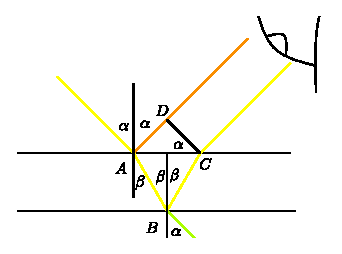
\includegraphics[width=1\linewidth]{img/o-03-1.eps}
	\caption{Интерференция в тонкой плёнке. $\alpha$ — угол падения, $\beta$ — угол преломления, жёлтый луч отстанет от оранжевого, они сводятся глазом в один и интерферируют.}
\end{figure}
Так, интерференция возникает при разделении первоначального луча света на два луча при его прохождении через тонкую плёнку, например плёнку, наносимую на поверхность линз у просветлённых объективов. Луч света длиной волны $\lambda$ , падая перпендикулярно к поверхности плёнки толщиной $d$, отразится дважды — от внутренней и наружной её поверхностей. Если пленка достаточно тонка, так что её толщина не превышает длину цуга волн падающего света, то на верхней границе раздела сред отражённые лучи будут когерентны и поэтому смогут интерферировать.

Изменение фазы проходящего через плёнку луча, в общем случае, зависит от показателя преломления плёнки и окружающих её сред. Кроме того, надо учитывать, что свет при отражении от оптически более плотной среды меняет свою фазу на половину периода. Так, например, в случае для воздуха ($n_1 ≈ 1$), окружающего тонкую масляную плёнку ($n_2 ≈ 1.5$), луч, отражённый от внешней поверхности будет иметь сдвиг фазы $\pi$ , а от внутренней — не будет. Интерференция будет конструктивной, если итоговая разница между пройденными этими лучами путями на поверхности плёнки будет составлять полуцелое число длин волн в плёнке $\lambda_2 = \lambda_1\frac{n_1}{n_2}$.\\
То есть\\
${\displaystyle \Delta \varphi _{const}=2d{\frac {2\pi }{\lambda _{2}}}+\pi (2k-1)=2d{\frac {2\pi n_{2}}{\lambda _{1}n_{1}}}+\pi (2k-1),k\in \mathbb {Z} }$\\ 
Для деструктивной интерференции в данном примере необходимо, чтобы разность фаз между лучами была кратна $2\pi$ .\\
То есть ${\displaystyle \Delta \varphi _{dest}=2d{\frac {2\pi n_{2}}{\lambda _{1}n_{1}}}+2\pi k,k\in \mathbb {Z} }$ \\
Полное гашение лучей произойдет для толщин пленки:\\
${\displaystyle d_{dest}={\frac {1}{2}}\lambda _{1}k{\frac {n_{1}}{n_{2}}}}$ 
Если ${\displaystyle \lambda _{1}=400}$ нм, то длина этой волны в масляной пленке ${\displaystyle \lambda _{2}=\lambda _{1}{\frac {n_{1}}{n_{2}}}=400{\frac {1}{1.5}}\approx 267}$ нм.

\textbf{Дополнение}\\
Рассмотрим частный случай электромаггнитых волн, когда поле зависит от одной координаты, скажем $x$(и от времени). Такие волны называются плоскими. В этом случае уравнения поля принимают вид:
\begin{gather}
\label{o-03-pole}
\frac{\partial^2f}{\partial t^2} - c^2\frac{\partial^2f}{\partial x^2} = 0,
\end{gather}
где $f$ - любая компонента векторов $E$ или $H$.\\ 
Решение данного уравнения имеет вид:
\begin{gather*}
f = f_1(\xi) + f_2(\eta),
\end{gather*}
где $f_1$ и $f_2$ - произвольные функции. Таким образом,
\begin{gather}
\label{o-03-f}
f = f_1(t - \frac{x}{c}) + f_2(t + \frac{x}{c}).
\end{gather}
Выберем потенциалы рассматриваемой плоской волны так, чтобы $\varphi = 0$, причём  $div A = 0$. Последнее условие даёт:
\begin{gather*}
\frac{\partial A_x}{\partial x} = 0,
\end{gather*}
поскольку все величины не зависят от $y$ и $z$. Согласно $\ref{o-03-pole}$ будем иметь тогда и $\frac{\partial^2A_x}{\partial t^2} = 0$, т.е. $\frac{\partial A_x}{\partial t} = const$. Но производная $\partial A/\partial t$ определяет электрическое поле, отличная от нуля компонента $A_x$ означала бы в рассматриваемом случае наличие постоянного продольного электрического поля. Поскольку такое поле не имеет отношения к электромагнитной волне, то можно положить $A_x = 0$.
Такиим образом, векторный потенциал плоской волны может быть всегда выбран перпендикулярным к оси $x$, т.е. к направлению распространения этой волны.\\
Рассмотрим плоскую волну, бегущую в положительном направлении оси $x$; в такой волне все величины, в частности и $A$, являются функциями только от $t - x/c$. Из формул
\begin{gather*}
E = -\frac{1}{c}\frac{\partial A}{\partial t}, \quad H = rot A
\end{gather*}
мы находим поэтому:
\begin{gather*}
E = -\frac{1}{c}A', \quad H = [\triangledown A] = [\triangledown (t - \frac{x}{c})\cdot A'] = -\frac{1}{c}[nA'],
\end{gather*}
где штрих обозначает дифференцирование по $t - x/c$, а $n$ - единичный вектор вдоль направления распространения волны. Подставляя первое равенство во второе, находим:
\begin{gather}
\label{o-03-H}
H = [nE].
\end{gather}
Мы видим, что электрическое и магнитное поля $E$ и $H$ плоской волны направлены перпендикулярно к направлению распространения волны. На этом основании электромагитные волны называют поперечными.\\
\end{document}